\begin{figure}[h]
\centering
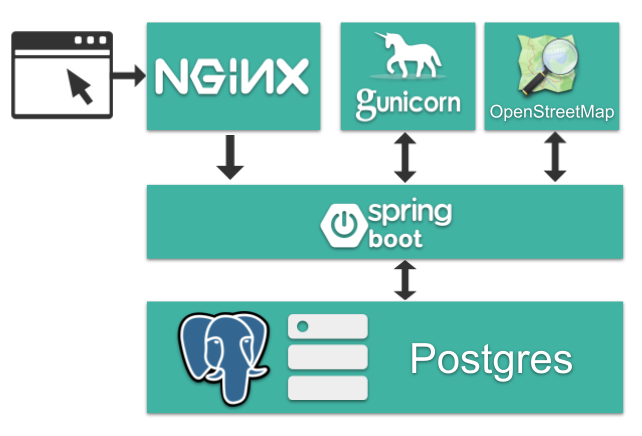
\includegraphics[width=0.5\textwidth]{TechStack.png}
\caption{Tech Stack implementation of the application} \label{TechStack}
\end{figure}
\subsection{In-Depth Semi-Structured Interviews}

We asked 20 participants to use our application and asked them several
questions to gather information about our user profiling technique and
timetable generator. The target audience of our interviews were of various
types. We found a balance between people who use social media frequently and
people who don't, who felt that their social media profile does not reflect
their itinerary preferences. First, the application generated two timetables. A
personalised itinerary and an itinerary where the travel interest vector is
ignored; therefore, all POIs have an equal chance of being selected. However,
the participants were not told which one was which, and we mixed the order of
timetables to avoid anchor bias. 


We first started discussing with what the interviewee looks
for in a holiday  so we
could check whether this matches their travel interest
vector. Then, after the timetables were generated, we
asked them to review the results and which timetable they
think was more personalised.  At this stage, the
interviewees were shown their automatically generated
characteristics and asked what they would change,
followed by whether they think their social media
presence represents their travel preferences.

Finally, we discussed some considerations and future
improvements regarding automatic preference gathering
from social media and how this approach differs from
their usual travel planning.
